\let\negmedspace\undefined
\let\negthickspace\undefined
\documentclass[journal]{IEEEtran}
\usepackage[a5paper, margin=10mm, onecolumn]{geometry}
%\usepackage{lmodern} % Ensure lmodern is loaded for pdflatex
\usepackage{tfrupee} % Include tfrupee package

\setlength{\headheight}{1cm} % Set the height of the header box
\setlength{\headsep}{0mm}     % Set the distance between the header box and the top of the text

\usepackage{gvv-book}
\usepackage{gvv}
\usepackage{cite}
\usepackage{amsmath,amssymb,amsfonts,amsthm}
\usepackage{algorithmic}
\usepackage{graphicx}
\usepackage{textcomp}
\usepackage{xcolor}
\usepackage{txfonts}
\usepackage{listings}
\usepackage{enumitem}
\usepackage{mathtools}
\usepackage{gensymb}
\usepackage{comment}
\usepackage[breaklinks=true]{hyperref}
\usepackage{tkz-euclide} 
\usepackage{listings}
% \usepackage{gvv}                                        
\def\inputGnumericTable{}                                 
\usepackage[latin1]{inputenc}                                
\usepackage{color}                                            
\usepackage{array}                                            
\usepackage{longtable}                                       
\usepackage{calc}                                             
\usepackage{multirow}                                         
\usepackage{hhline}                                           
\usepackage{ifthen}                                           
\usepackage{lscape}
\begin{document}

\bibliographystyle{IEEEtran}
\vspace{3cm}

\title{1}
\author{EE23BTECH11063 - Vemula Siddhartha
}
% \maketitle
% \newpage
% \bigskip
{\let\newpage\relax\maketitle}

\renewcommand{\thefigure}{\theenumi}
\renewcommand{\thetable}{\theenumi}
\setlength{\intextsep}{10pt} % Space between text and floats


\numberwithin{equation}{enumi}
\numberwithin{figure}{enumi}
\renewcommand{\thetable}{\theenumi}


\textbf{Question}:\\
If the sum of first 7 terms of an AP is 49 and that of 17 terms is 289, find the sum of
first n terms.
\\
\textbf{Solution: }
\begin{table}[h!]    
  \centering
  \begin{tabular}[12pt]{ |c| c|}
    \hline
    \textbf{Variable} & \textbf{Description}\\ 
    \hline
    $x\brak{0}$ & First term of the AP \\
    \hline 
    $d$ & Common difference of the AP\\
    \hline
    $y\brak{n}$ & Sum of $n+1$ terms of the AP\\
    \hline
    $x\brak{n}$ & General term\\
    \hline   
    \end{tabular}
  \caption{Variables Used}
  \label{tab10.5.3.9.1}
\end{table}
\begin{align}
y\brak{n}&=\frac{n+1}{2}\,\brak{2x\brak{0}+nd}\,u\brak{n}\label{eq10.5.3.9.1}\\
y\brak{6}&=49\\
y\brak{16}&=289
\end{align}
Then,
\begin{align}
x\brak{0}+3d&=7\label{eq10.5.3.9.2}\\
x\brak{0}+8d&=17 \label{eq10.5.3.9.3}
\end{align}
From  equations \ref{eq10.5.3.9.2} and \ref{eq10.5.3.9.3}, the augmented matrix is:
\begin{align}
 \myvec{
   1 & 3 & 7
   \\
   1 & 8 & 17
 }
 \xleftrightarrow[]{R_2 \leftarrow {R_2-R_1}}
 \myvec{
   1 & 3 & 7
   \\
   0 & 5 & 10
 }
 \\
 \xleftrightarrow[]{R_1 \leftarrow {R_1-\frac{3}{5}R_2}}
 \myvec{
   1 & 0 & 1
   \\
   0 & 5 & 10
 }
 \\
 \xleftrightarrow[]{R_2 \leftarrow \frac{R_2}{5}}
 \myvec{
   1 & 0 & 1
   \\
   0 & 1 & 2
 }
 \\
 \implies \myvec{
   x\brak{0}
   \\
   d
 }
 =
 \myvec{
   1
   \\
   2
 }
\end{align}
\begin{align}
    x\brak{n}&= \brak{1+2n}u\brak{n}\\
    X\brak{z}&=\frac{1}{1-z^{-1}}+\frac{2z^{-1}}{\brak{1-z^{-1}}^2}\;\;\cbrak{z\in\mathbb{C}: |z|>1}
\end{align}
\begin{align}
   y\brak{n}&=x\brak{n}*u\brak{n}\\
   Y\brak{z}&=X\brak{z}\,U\brak{z}\\
   \implies Y\brak{z}&=\brak{\frac{1}{1-z^{-1}}+\frac{2z^{-1}}{\brak{1-z^{-1}}^2}}\brak{\frac{1}{1-z^{-1}}}\\
   &=\frac{1}{\brak{1-z^{-1}}^2}+\frac{2z^{-1}}{\brak{1-z^{-1}}^3}\\
   \brak{n+1}u\brak{n}&\system{Z}\frac{1}{\brak{1-z^{-1}}^2}\cbrak{z\in\mathbb{C}: |z|>1}\\
   n\brak{\brak{n+1}u\brak{n}}&\system{Z}\frac{2z^{-1}}{\brak{1-z^{-1}}^3}\cbrak{z\in\mathbb{C}: |z|>1}
\end{align}
   From equations \eqref{eq:uzder-shift} and \eqref{eq:uzder-der}, taking the inverse Z Transform,
   \begin{align}
   y\brak{n}&=\brak{n+1}u\brak{n}+n\brak{\brak{n+1}u\brak{n}}\\
   \implies y\brak{n}&=\brak{n+1}^2\,u\brak{n}
\end{align}
\begin{figure}[h!]
   \centering
   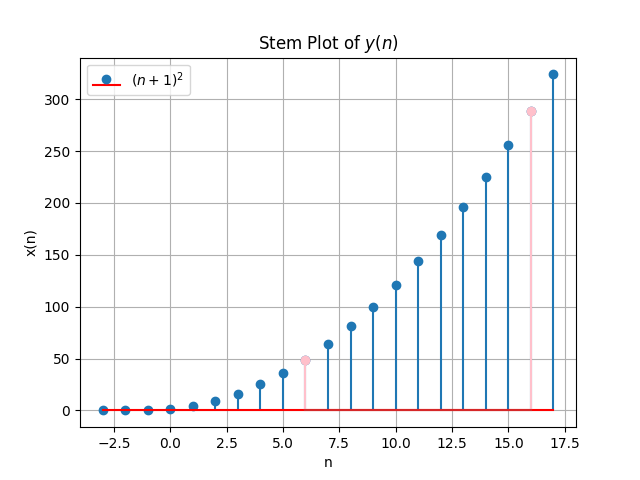
\includegraphics[width=0.7\linewidth]{figs/Figure_1.png}
   \caption{Stem Plot of y\brak{n}}
   \label{stemplot}
\end{figure}
\end{document}  
\end{document}


